% =====================================================================
% PCR-Net: Command-Space Conflict Arbitration for Hexapod Target
% Following in Clutter. IEEE conference-format draft (pdflatex).
% Figures: PDF vector graphics in figs/.
% Author info and publication metadata should be checked before submission.
% =====================================================================
\documentclass[letterpaper, 10 pt, conference]{ieeeconf}
\IEEEoverridecommandlockouts
\overrideIEEEmargins
\usepackage{amsmath,amssymb,amsfonts}
\usepackage{graphicx}
\usepackage{stfloats}
\usepackage{booktabs}
\usepackage{multirow}
\usepackage{array}
\usepackage{algorithm}
\usepackage{algpseudocode}
\usepackage{xcolor}
\usepackage{url}
\usepackage{pifont}
\usepackage[hidelinks]{hyperref}
% w = learned conflict prior (GatePolicy output), NOT angular velocity;
% the yaw command component is $u_\omega$. See notation_table.md.
\newcommand{\uF}{u_{F}}
\newcommand{\uA}{u_{A}}
\newcommand{\yeff}{y_{\mathrm{eff}}}
\newcommand{\rFdir}{\rho_F}
\newcommand{\rAdir}{\rho_A}
\newcommand{\dyrdir}{\Delta y_r}
\newcommand{\msec}{\,\mathrm{m/s}}
\newcommand{\ms}[2]{\ensuremath{#1{\pm}#2}}
\newcommand{\bms}[2]{\ensuremath{\mathbf{#1{\pm}#2}}}

\begin{document}
\title{\LARGE \bf
PCR-Net: Command-Space Conflict Arbitration for\\
Hexapod Target Following in Clutter}
\author{
\thanks{}%
\thanks{}}
\maketitle
\thispagestyle{empty}
\pagestyle{empty}

\begin{abstract}
Target following in clutter is not merely tracking a moving waypoint: the
target's traversable space can differ from the robot's. For a legged robot,
this passability mismatch turns local following into a command-space
arbitration problem, because the command that preserves following can
be incompatible with the command that keeps the robot collision-free.
PCR-Net formulates this conflict as continuous arbitration within a single
executable velocity command, rather than a switch between separate behaviors.
It decomposes the command into Follow and Avoid proposals and fuses them
through a risk-conditioned learned gate on top of a fixed low-level locomotion
policy. On a controlled target-following benchmark in structured clutter,
PCR-Net sustains $0.95$ task success at an above-training target speed,
while rule-based, structural, learning-based, and planner-style alternatives expose
distinct safety--following failure modes. A checkpoint-controlled inference
ablation shows that the learned correction supports target
retention during high-conflict maneuvers. Across $60$ real-robot trials,
PCR-Net succeeds in $37/40$ runs, compared with $12/20$ for Rule-Override,
using onboard target detection and stereo-depth maps in corridor clutter.
\end{abstract}

\section{Introduction}
A legged robot following a moving person faces a difficulty that is
especially acute for a finite-bodied platform with gait dynamics:
\emph{the target's passability is not the robot's safe passability}
(Fig.~\ref{fig:teaser}). A person can turn sideways through a narrow gap or
step between obstacles, whereas the robot's wider gait envelope cannot safely
reproduce the same path. The path that keeps the robot closest to the person may lead
it into an obstacle, while the path that keeps it safe may cause it to
lose the person. The task is therefore neither pure obstacle avoidance
nor pure target tracking.

We study this difficulty as a conflict in the robot's \emph{command
space}. At each control step the high-level controller emits one velocity
command. The command that best maintains following and the command that
best avoids collision can become incompatible---competing for command
authority within that single output. Standard local navigation formulations
that treat the target only as a moving waypoint do not explicitly
preserve target tracking during local avoidance, and
fixed-priority switching between a follow and an avoid behavior can lose
the target during the maneuver. We therefore study an arbitration that
reconciles the two objectives within a single command at every instant,
and compare it with arbitration ablations, a structural variant,
a monolithic learned policy, and a planner-style velocity search.

PCR-Net addresses this conflict directly in the robot's command space
(Fig.~\ref{fig:system}). It treats the analytic Follow expert and the
learned Avoid expert as command proposals in orthogonal subspaces, then
uses a learned gate to produce one executable fusion---neither a hard
switch nor a predicted detour---conditioned on a per-command risk. The
risk is a command-direction-conditioned local clearance prior, not a
prediction of the world; it informs the gate rather than deciding for it.
All arbitration runs on top of a fixed, pretrained low-level locomotion
policy shared by every compared method.
\begin{figure}[t]
\centering
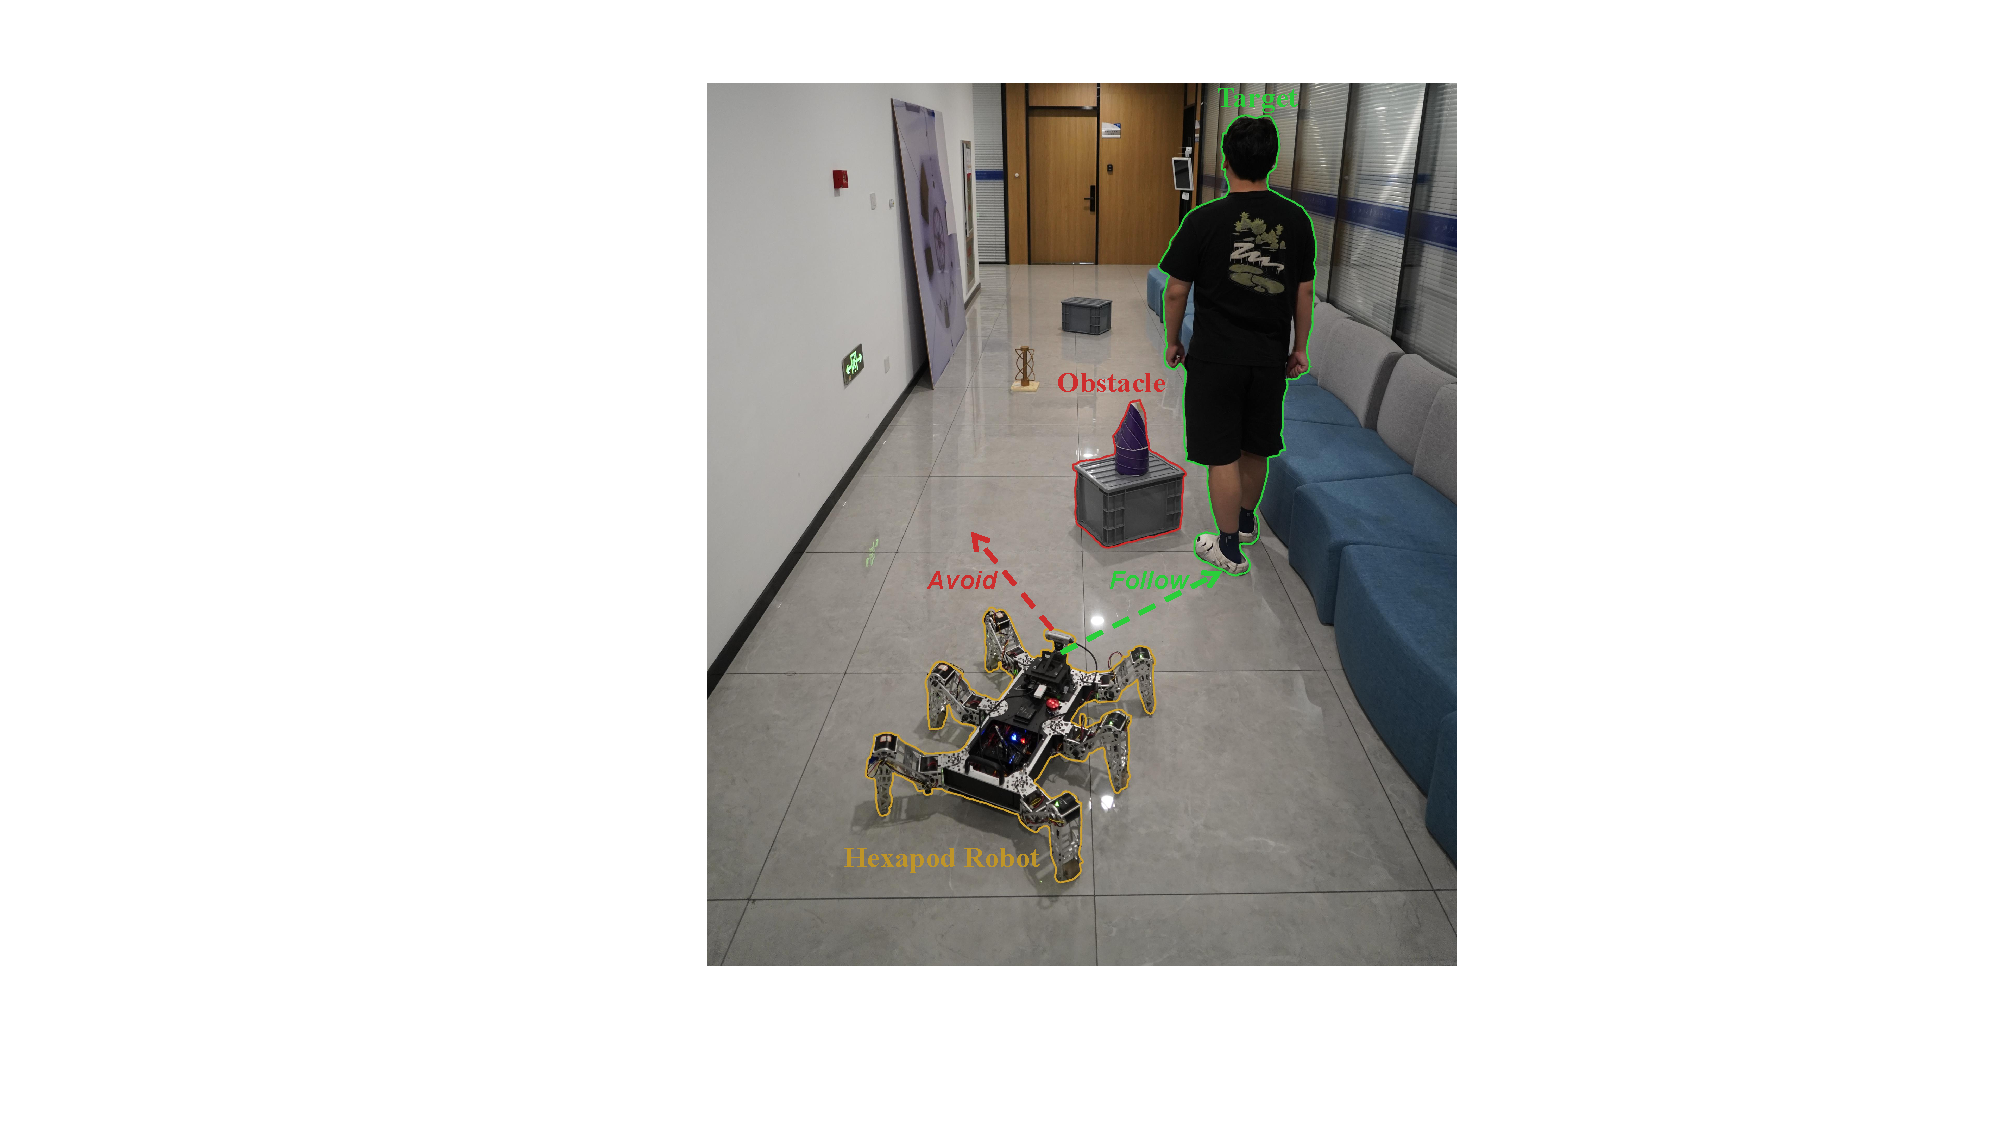
\includegraphics[width=0.80\columnwidth]{figs/fig1_real_scene.pdf}
\caption{Real corridor setting for hexapod target following in clutter.
The target can pass through narrow gaps that are not safely replicable by
the robot's leg-inclusive safety envelope, creating a command-space conflict
between target recovery and collision avoidance.}
\label{fig:teaser}
\end{figure}
The hexapod platform is a useful testbed for this arbitration problem:
omnidirectional stepping makes lateral sidestepping natural, while each
command must still be realized by a fixed 18-joint locomotion policy rather
than a perfect velocity-controlled base.

Although command-space conflict is not specific to row geometries, we use
staggered rows as a controlled stress test: alternating narrow gaps repeatedly
require lateral avoidance while the target advances, isolating the arbitration
problem for systematic ablation.

\noindent\textbf{Contributions.} This work makes three contributions.
\begin{itemize}
\item \textbf{Command-space reframing of target following in clutter.} We
formulate following in structured clutter as a command-level conflict
between target-preserving and collision-avoiding motion, and instantiate
it through an orthogonal Follow/Avoid command decomposition whose
structural properties keep the arbitration bounded and interpretable.
\item \textbf{Risk-conditioned soft arbitration for hexapod following.} We
propose PCR-Net, a high-level module that couples per-command risk with
context-dependent fusion of the Follow and Avoid commands while using a
fixed low-level locomotion policy.
\item \textbf{Controlled validation against rule-based, structural,
learning, and planner-style alternatives.} Through simulation ablations,
an additive-fusion variant, a monolithic policy, and a DWA-style velocity
search, together with a quantitative hexapod deployment, we characterize
the resulting safety--following trade-offs and show that learned
arbitration achieves the most favorable safety--following balance among
the tested alternatives in our benchmark.
\end{itemize}

\section{Related Work}
\emph{Following, avoidance, and agile locomotion.}
Early follow-and-avoid systems separate the two behaviors with hand-tuned
priorities or finite-state logic, and person-following is largely framed as
mobile-robot tracking and local navigation~\cite{ref:personfollowing}. Closest
in setting, obstacle-avoidant quadruped leader following has been studied with
navigation-centric designs~\cite{ref:leaderfollow}. We instead isolate
the continuous command-space arbitration needed by a legged follower under
passability mismatch. Recent learned legged controllers achieve agile avoidance
and robust perceptive locomotion by coupling control with local
navigation~\cite{ref:abs,ref:miki}: He et al.~\cite{ref:abs}
switch an agile and a recovery policy through a learned reach-avoid value for
collision-free high-speed motion toward a \emph{static} goal. We follow a
\emph{moving} person through clutter, where the difficulty is preserving
tracking during avoidance, and we fuse continuously rather than switching
discretely.

\emph{Planning, safety, and expert arbitration.}
Dynamic-window and velocity-space methods~\cite{ref:dwa} score
short-horizon rollouts against clearance and progress costs; we adapt a
DWA-style target-aware search as a planner-style alternative
(Sec.~\ref{sec:external}), sharing our map, velocity limits, and low-level
stack but with a fixed hand-designed cost. Task-priority and null-space
control allocate lower-priority objectives to residual freedom
~\cite{ref:taskpriority}, while control-barrier-function QPs encode safety
constraints in online optimization~\cite{ref:cbf}. Reach-avoid value
learning~\cite{ref:reachavoid} provides a safety-oriented alternative, while
mixture-of-experts models provide a classical mechanism for gated expert
composition~\cite{ref:moe}, and shared-autonomy methods contextualize policy
blending~\cite{ref:policyblend}. Residual policy learning augments nominal
control with a learned action correction~\cite{ref:residualrl}; PCR-Net instead
confines the residual to the scalar arbitration coordinate between fixed
expert proposals. Here the human is the moving target; PCR-Net uses
command-direction-conditioned clearance as a prior for a learned
gate, and resolves the conflict by continuous fusion rather than by switching,
null-space projection, or trajectory search.

\section{Problem Formulation}
\textbf{A. Setting.}
We instantiate the general clutter-following problem in a representative
staggered-row layout (Fig.~\ref{fig:teaser}), where alternating gaps
repeatedly expose the passability mismatch. The
high-level controller outputs a velocity command
$u=[u_x,u_y,u_\omega]^\top$ (lateral, forward, yaw) at $10\,\mathrm{Hz}$,
realized by a fixed low-level locomotion policy at $50\,\mathrm{Hz}$. The
robot perceives a local affordance map and the relative target state; it
has no global map.

\textbf{B. Orthogonal command decomposition.}
We assign following and avoidance to orthogonal command subspaces. The
Follow expert acts in the forward--yaw subspace and the Avoid expert in
the lateral subspace,
\begin{equation}
\mathcal{U}_F=\{[0,u_y,u_\omega]^\top\},\quad
\mathcal{U}_A=\{[u_x,0,0]^\top\},
\end{equation}
so that $\mathbb{R}^3=\mathcal{U}_F\oplus\mathcal{U}_A$ and
$\mathcal{U}_F\perp\mathcal{U}_A$. A Follow command
$\uF=[0,u_{F,y},u_{F,\omega}]\in\mathcal{U}_F$ is computed analytically;
the learned Avoid expert produces a raw command projected onto the
lateral subspace, $\uA=[u_{A,x},0,0]\in\mathcal{U}_A$. Because yaw lies in
the Follow subspace, a nonzero following weight preserves part of the
target-oriented yaw during lateral avoidance, helping the robot keep facing
the target while it sidesteps; whether the target is actually retained is
examined empirically in Sec.~\ref{sec:results}.

\textbf{C. The conflict.}
When the target passes through an obstacle configuration the robot cannot
replicate, the following-optimal command (along $\uF$) and the
avoidance-optimal command (along $\uA$) lie in orthogonal subspaces, and
a single command generally cannot maximize both target recovery and
immediate clearance. The controller must therefore \emph{arbitrate}
between them rather than select one.

\textbf{D. Task success and diagnostics.}
We separate event success from trajectory diagnostics. A trial succeeds only
if, at the success event, the robot has cleared the final obstacle row, lies
within the follow band, and has stayed collision-free over the episode. We
then report trajectory diagnostics: follow MAE (mean
$|\mathrm{dist}(\text{target},\text{robot})-d_{\mathrm{des}}|$ over
high-level steps), L1 (no collision), L2 (target retained: follow MAE
$\le 0.5\,\mathrm{m}$ and in-FOV $\ge 0.90$), and L3 (final-row
clearance). L1/L2/L3 are not additional success requirements; a successful
trial can have MAE above $0.5\,\mathrm{m}$ if transient errors occur during
obstacle negotiation and the robot recovers before the event (Sec.~\ref{sec:results}-A).

\begin{figure*}[t]
\centering
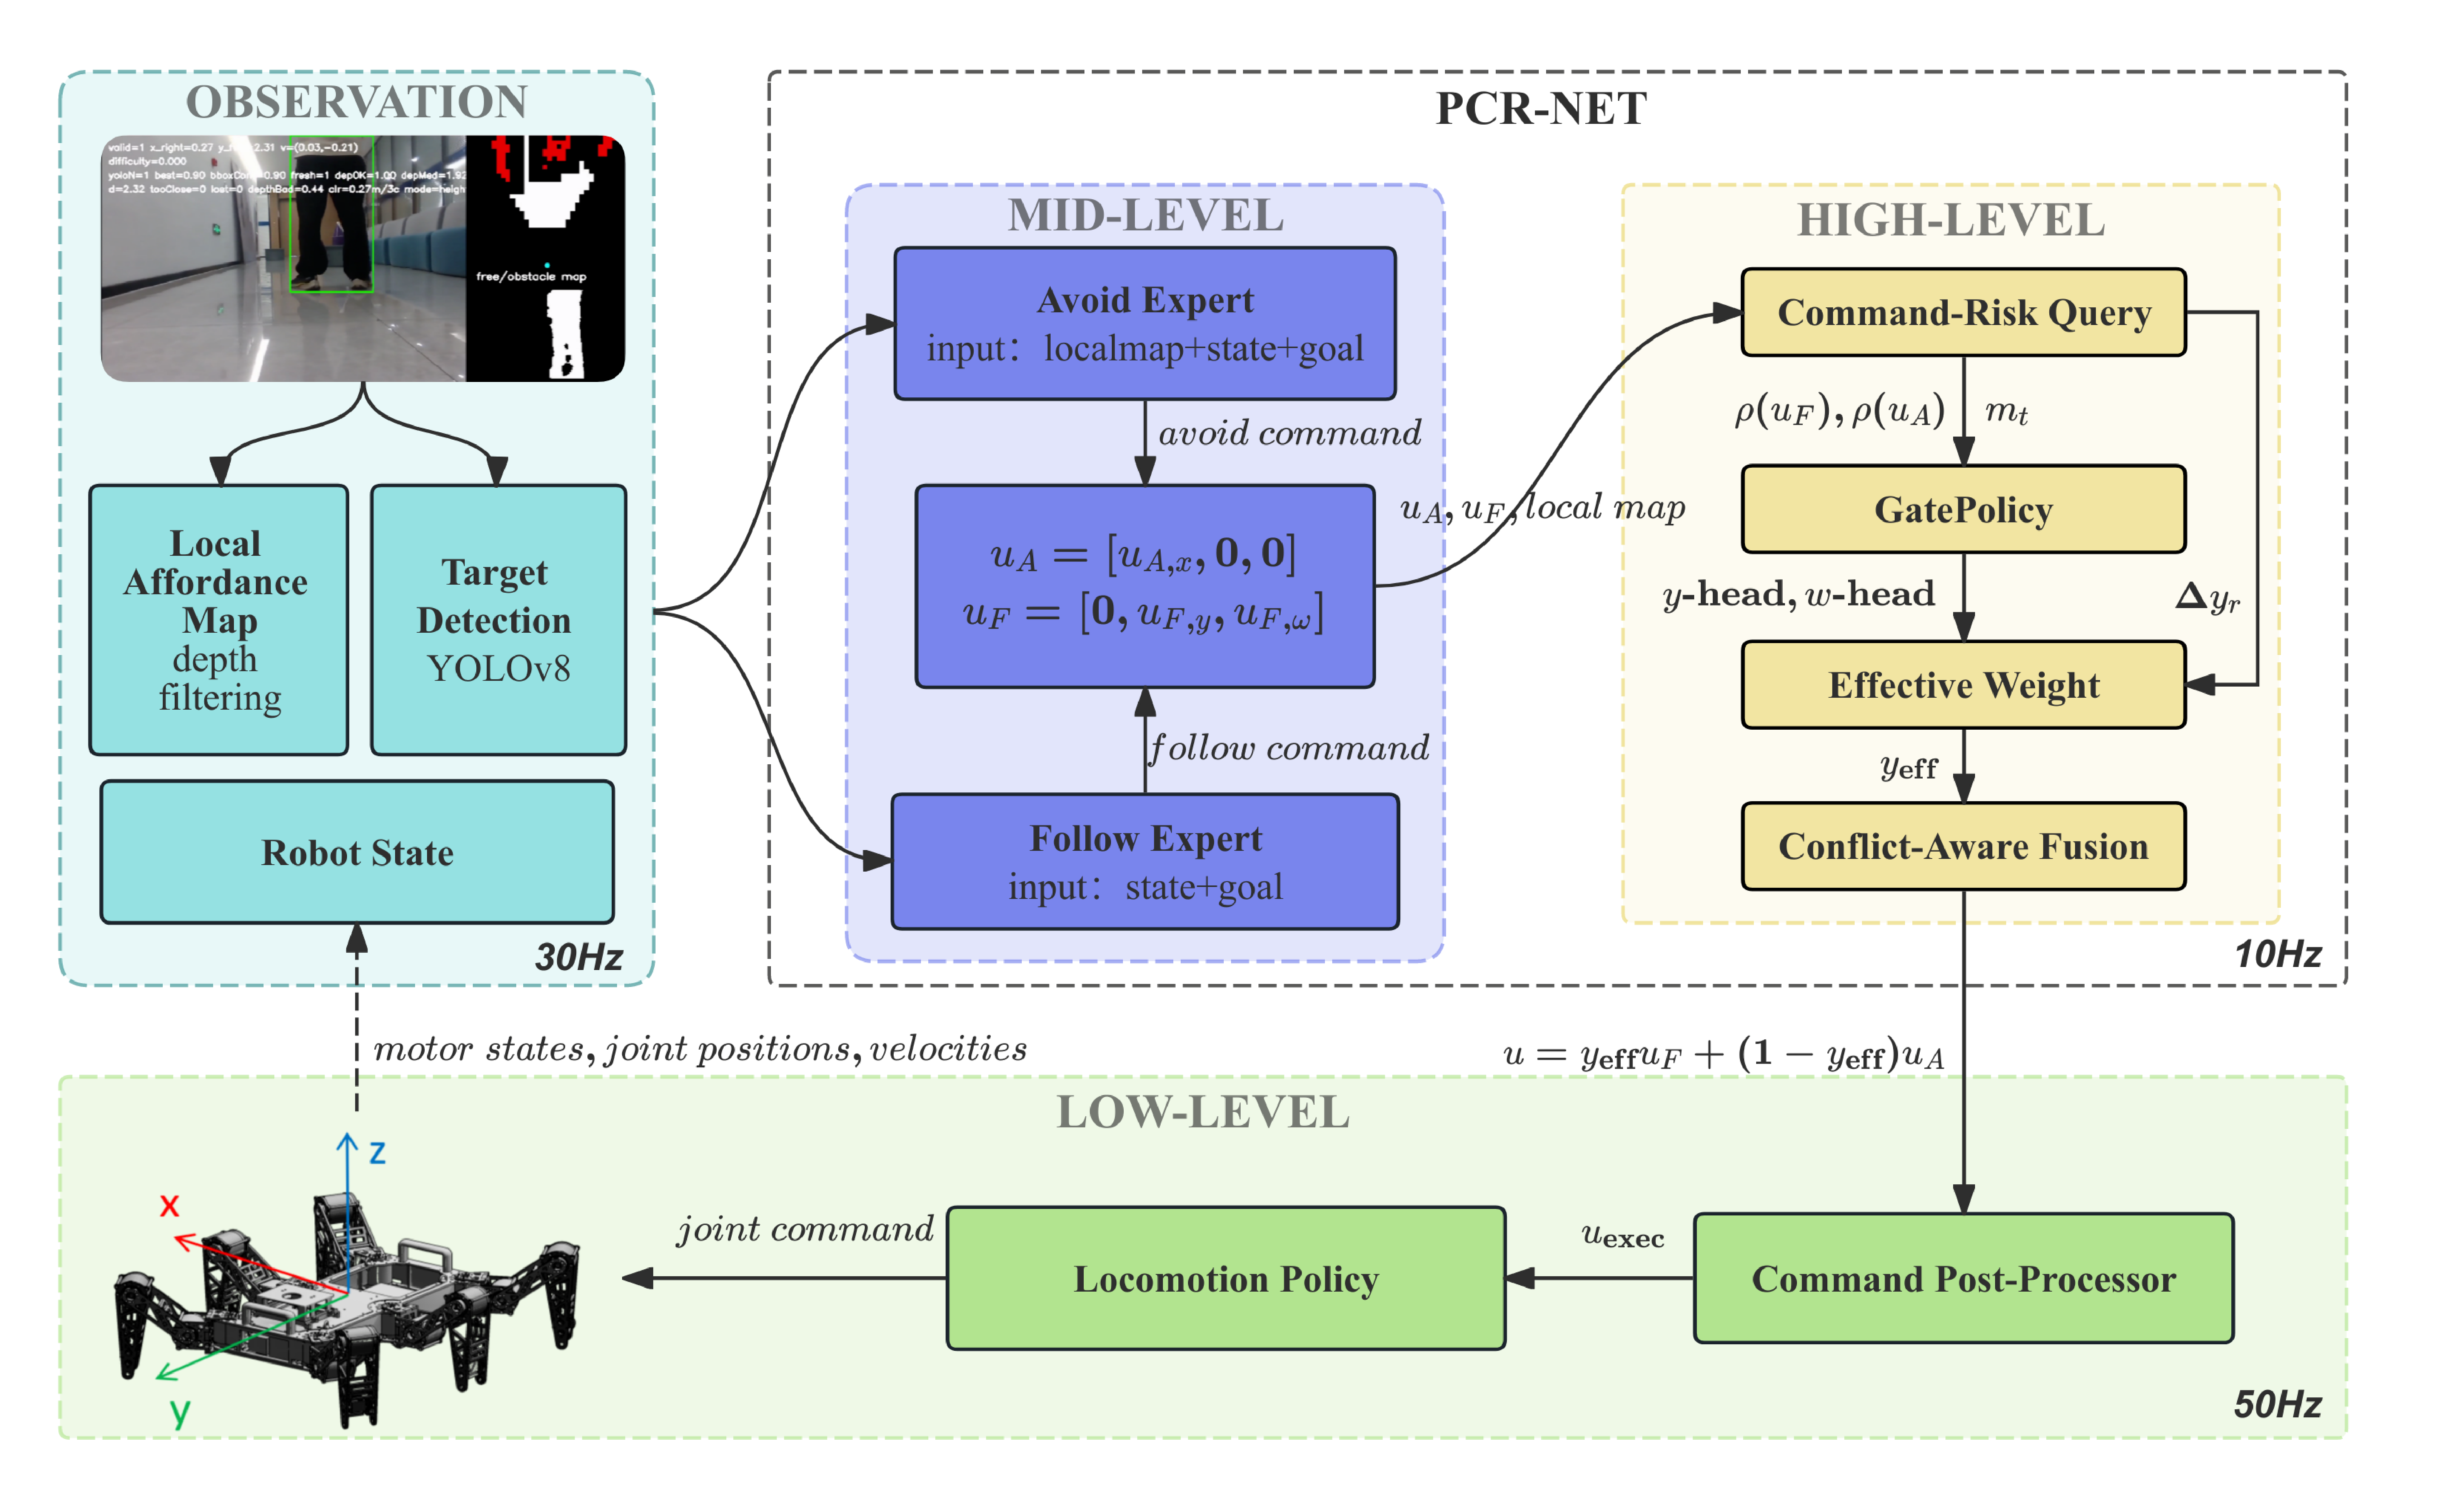
\includegraphics[width=0.90\textwidth]{figs/fig1_system.pdf}
\caption{PCR-Net command-space arbitration. Onboard perception supplies a
local occupancy--clearance map and relative target state
(YOLOv8~\cite{ref:yolo}). The analytic Follow expert proposes forward--yaw
motion, the learned Avoid expert proposes lateral motion, and
command-conditioned risks inform a learned gate that computes $\yeff$ and
blends the two proposals. A shared fixed locomotion policy tracks the shaped
command. Rates indicate deployment frequencies: onboard perception updates at
30 Hz, arbitration runs at 10 Hz, and the fixed locomotion policy tracks
commands at 50 Hz.}
\label{fig:system}
\end{figure*}

\section{Method}
\label{sec:method}
PCR-Net is a three-level hierarchy (Fig.~\ref{fig:system}): a fixed
locomotion policy tracks velocity commands, two experts propose commands in
orthogonal subspaces, and a risk-conditioned gate fuses them into one
executable command.

\textbf{A. Follow expert (analytic).}
The Follow expert computes $\uF=[0,u_{F,y},u_{F,\omega}]$ analytically
from the relative goal, using a turn-in-place-then-advance rule with
hysteresis: when the bearing exceeds $0.35\,\mathrm{rad}$ the forward term
is suppressed and the robot turns in place; it resumes advancing once the
bearing falls below $0.18\,\mathrm{rad}$.

\textbf{B. Avoid expert (learned).}
The Avoid expert takes the local affordance map, robot state, and relative
goal, and produces a raw three-dimensional command projected onto the
lateral subspace ($\uA$) before arbitration. It is pretrained in the
structured obstacle-row scenes and then frozen (Sec.~IV-F), so all
arbitration methods share the same avoidance capability.

\textbf{C. Per-command risk (PCR).}
For a candidate command $u$, we evaluate a risk by a cone query on the
local affordance map $M_t$ ($32\times32$ cells, $0.09375\,\mathrm{m}$ per
cell, channels: occupancy and a clearance proxy). Along the command
bearing $\mathrm{atan2}(u_x,u_y)$ we open a cone of half-angle $25^\circ$
and take the minimum clearance $d$ within it ($d=3.0\,\mathrm{m}$ if no
obstacle). The risk is
\begin{equation}
\rho(u)=1-\mathrm{clip}\!\left(\tfrac{d-d_{\mathrm{safe}}}
{d_{\mathrm{free}}-d_{\mathrm{safe}}},0,1\right),
\end{equation}
with $d_{\mathrm{safe}}=0.27\,\mathrm{m}$, $d_{\mathrm{free}}=0.57\,
\mathrm{m}$; we evaluate the directional gate risks
$\rFdir=\rho(\uF)$ and $\rAdir=\rho(\uA)$. This $\rho$ is a
\emph{command-direction-conditioned clearance prior}: it depends on the
command bearing and the nearest occupied cell in the cone rather than a
predicted trajectory. The prior is direction-conditioned rather than
speed-aware. As a sensitivity check, we also evaluate
$\rho_v(u)=\rho(u)\min(1,v_{\mathrm{cmd}}/v_{\max})$, where
$v_{\mathrm{cmd}}=\|[u_x,u_y]\|_2$. This speed-scaled variant produces only
marginal differences over $0.35$--$0.60\msec$, supporting the simpler
directional form in the tested low-speed regime.

\emph{Distance-decayed risk memory.} To retain awareness of a hazard that
briefly leaves the field of view, we maintain a risk memory that decays
with measured forward body motion rather than elapsed time (it does not
decay during purely lateral motion or while stopped):
\begin{equation}
\begin{aligned}
m_t &= \max\!\big(\rho_{F,t},\,m_{t-1}e^{-\Delta s/L_{\mathrm{clear}}}\big),\\
\Delta s &= \max(v_{y,t}^{\mathrm{body}},0)\,\Delta t ,
\end{aligned}
\end{equation}
with $L_{\mathrm{clear}}=0.40\,\mathrm{m}$. The risk memory is a temporal
feature supplied to the gate; it does not replace the instantaneous risks
$\rFdir,\rAdir$ used by the analytic correction below.

\textbf{D. Gate and conflict-aware fusion.}
A single GatePolicy uses Beta heads for the base following weight $y$ and
learned conflict variable $w\in(0,1)$, matching their bounded semantics while
allowing state-dependent concentration; the centered transform of $w$ gives
the signed modulation $\Delta y_w$. It encodes the local
affordance map, robot state, relative goal, and the command-conditioned
features (the candidate commands
$\uF,\uA$ and their difference, the per-command risks $\rFdir,\rAdir$,
clearances, command cosine, conflict score, and risk memory). The
symbol $y$ denotes this scalar following gate, whereas $u_y$ denotes the
forward component of a velocity command. The effective following weight
combines a learned and an analytic correction,
\begin{align}
\Delta y_w &= \lambda\,\mathrm{deadband}(2w-1),\quad
\dyrdir = \gamma(\rAdir-\rFdir), \\
\yeff &= \mathrm{clip}\!\left(y+\Delta y_w+\dyrdir,\,0,\,1\right),
\end{align}
with $\lambda=0.30$, $\gamma=0.15$, and
$\mathrm{deadband}(z)=z$ for $|z|>0.05$ and $0$ otherwise. The fused
command is the convex blend
\begin{equation}
u = \yeff\,\uF + (1-\yeff)\,\uA .
\label{eq:fusion}
\end{equation}
Values $w>0.5$ reinforce following, whereas $w<0.5$ suppresses it through
the signed correction $\Delta y_w$. This correction is monotone non-decreasing in
its effect on $\yeff$: $\partial\yeff/\partial w=2\lambda=0.60$ in the
active unsaturated region, and $0$ inside the dead-zone or after clipping.
The two corrections play distinct roles: $\dyrdir$ is an analytic
directional risk-difference term, while $\Delta y_w$ is a learned signed
modulation.
The naming follows the gate's configuration: with only the $y$-head the
gate reduces to the \emph{Y-only} baseline; adding the $w$-head and the
command-conflict features yields the \emph{Learned-w} model, our PCR-Net.

\textbf{E. Low-level locomotion interface.}
The high-level command is emitted at $10\,\mathrm{Hz}$ and tracked by a
fixed locomotion policy at $50\,\mathrm{Hz}$. The low-level policy is
shared by all compared methods and is never updated during arbitration
training; it executes velocity commands but makes no avoidance or
following decision. Before reaching it, every method's fused command
passes through the same fixed shaping stage (amplitude clamping,
slew-rate limiting, clearance-based scaling); because this stage and the
low-level policy are identical across methods, they do not confound the
attribution of performance differences.

\textbf{F. Training procedure.}
Training proceeds in stages (Fig.~\ref{fig:system}, bottom to top).
First, we pretrain a velocity-conditioned hexapod locomotion policy with
RSL-RL~\cite{ref:rudin}, mapping high-level velocity commands to joint
actions; it is shaped for camera stability and impact smoothness, and is
frozen thereafter. Second, we train the Avoid expert alone in the
structured obstacle-row scenes to produce a safe lateral command from the
local occupancy--clearance map and the relative goal; it is then frozen.
The Follow expert uses no network, generating its candidate command
analytically. With the experts fixed, we train only the arbitration gate:
at each step the experts generate candidates, and the gate fuses them
using the local map, target state, command conflict, and per-command
risk. The final Learned-w model additionally learns the
command-conditioned conflict prior $w$ that corrects the base following
weight. A $0.05$-weighted binary-cross-entropy auxiliary term on the $w$
head favors $w=0$ on high-confidence avoidance states:
row-unreleased cases satisfying $\rFdir>0.25$,
$\rFdir-\rAdir>0.05$, and command cosine $<0.5$, plus a stricter global
fallback with higher risk and margin thresholds. Thus, the centered transform
of $w$ serves as a signed, context-dependent correction: it can reinforce or
compensate the analytic risk term $\dyrdir$ rather than acting as a
one-directional avoidance trigger; its realized sign is examined in the
hardware trace. No expert or low-level policy is jointly
fine-tuned, so all arbitration methods share identical expert and
locomotion capability.

The gate is trained with PPO~\cite{ref:ppo} in Isaac Gym~\cite{ref:isaac}
over a two-dimensional curriculum of target speed and obstacle-row count.
Each episode samples one of four levels---two rows at
$0.25$--$0.40\msec$, two rows at $0.35$--$0.50\msec$, three rows at
$0.30$--$0.50\msec$, and four-to-five rows at $0.35$--$0.50\msec$---with
the target speed held constant within an episode. Over $120{,}000$
episodes the sampling shifts from easier to harder levels while retaining
a fraction of easy episodes to reduce forgetting. Each obstacle stage has
complementary left-first and right-first zigzag layouts; at every reset a
layout is chosen reproducibly and each obstacle is perturbed by up to
$0.06\,\mathrm{m}$ along both horizontal axes, rejecting perturbations
that violate passage feasibility. Training obstacles are fixed cylinders
($0.15\,\mathrm{m}$ radius, $0.50\,\mathrm{m}$ height); contact friction
is randomized in $[0.4,0.8]$, with no mass, push, gravity, or actuator
randomization. The policy input during training is an actor-rasterized
occupancy--clearance map restricted to the D435i stereo FOV rather than
rendered depth.
The gate input is a two-channel occupancy--clearance map plus 13 robot-state scalars,
two target-state scalars, and 16 conflict features; encoders feed a
$256$--$256$ ELU trunk with Beta heads for $y$ and $w$. PPO uses 256 envs,
48 steps/iteration, five epochs, minibatch 12288, learning rate
$6{\times}10^{-5}$, entropy 0.04, clip 0.05, and 1000 iterations. Main
reward terms are row progress, follow distance, success, collision/terminal
penalties, and the $w$ auxiliary term.

\textbf{G. Arbitration design rationale.}
The command risk is used as a clearance prior rather than a reach-avoid
value, and unlike CBF-based controllers it does not provide a formal
forward-invariance certificate. Instead, three design choices keep the
one-step fusion bounded and interpretable. \emph{(i)} The Follow and Avoid
subspaces form an orthogonal direct sum
($\mathbb{R}^3=\mathcal{U}_F\oplus\mathcal{U}_A$), so following and lateral
avoidance are separable and no command axis is lost; for given $(\uF,\uA)$
the output is a one-dimensional convex trade-off, not an arbitrary vector.
\emph{(ii)} For any $\yeff\in[0,1]$ the fused command~\eqref{eq:fusion} lies
in the convex hull of $\{\uF,\uA\}$, so PCR-Net never extrapolates beyond
the two proposals, unlike a per-axis gate or additive fusion
(Sec.~\ref{sec:results}-C). \emph{(iii)} The fusion is a residual policy on
the convex expert segment. Let
$u_{\mathrm{nom}}=y\uF+(1-y)\uA$ denote the nominal command and
$\delta u=u-u_{\mathrm{nom}}$. Then
\begin{equation}
\delta u=(\yeff-y)(\uF-\uA),\quad
\|\delta u\|\le(\lambda+\gamma)\|\uF-\uA\|.
\label{eq:residual_bound}
\end{equation}
Thus, corrections are disagreement-aligned, vanish at coincident proposals,
and have bounded authority during conflict. PCR-Net therefore implements
bounded residual policy blending over a convex expert segment.

\section{Experiments}
\textbf{A. Setup.}
We evaluate on the fixed hardest stage (five rows, 13 capsule slots,
minimum passage width $0.75\,\mathrm{m}$, close to the robot's
$\sim0.65\,\mathrm{m}$ leg-inclusive safety envelope) and sweep three discrete target
speeds $\{0.35,0.50,0.60\}\msec$. The first two lie within the training
range; $0.60\msec$ is above the maximum training speed of $0.50\msec$, so
the high-conflict condition is an above-training speed-extrapolation
evaluation. Main arbitration results are mean $\pm$ std over three randomized
evaluation runs of 128 episodes each (384 episodes per method--speed
setting), with a 50-s episode horizon, on the fixed hardest stage. The inference ablation and DWA-style search
use that stage; monolithic PPO is evaluated over increasing row difficulty.
The hexapod model has $18$ actuated joints, a
$0.20\times0.44\times0.05\,\mathrm{m}$ body collision box, leg-link lengths
$0.072/0.13/0.17\,\mathrm{m}$, and a $0.25\,\mathrm{m}$ row-passing body
half-length; the D435i stereo camera is mounted at $(0,0.22,0.08)\,\mathrm{m}$ in the body
frame with $0^\circ$ pitch, $20^\circ$ roll, $90^\circ$ yaw,
$87^\circ\times58^\circ$ depth FOV, and $0.28$--$3.0\,\mathrm{m}$ range.
Simulation uses structured arrangements of regular geometric obstacle
primitives in Isaac Gym.

\textbf{B. Compared methods.}
We organize the comparison into three groups.
\emph{(1) Arbitration ablations} share the experts, observations, and
execution stack but apply different arbitration rules:
\emph{Y-only} ($\yeff=y$, no risk or learned modulation);
\emph{Geom-w}, a geometric clearance heuristic
$w_{\mathrm{geom}}=e^{-d/\tau}$ using the Follow-command clearance $d$ and
$\tau=0.15\,\mathrm{m}$, with $\yeff=y(1-w_{\mathrm{geom}})$;
\emph{Risk-only}, the analytic $\dyrdir$ term only, retrained from
scratch with no learned-$w$ head; \emph{Rule-Override}, a reactive
override on $\rFdir-\rAdir$ that forces lateral avoidance by cutting the forward
command to as low as $10\%$ while retaining up to $70\%$ of the yaw
command, using one fixed parameter set across all speeds; and
\emph{Learned-w}, the full PCR-Net.
\emph{(2) Structural alternative.} \emph{Additive-Fusion} replaces the
gate with direct command addition, $u=\uF+\uA$, keeping the same experts
but with no gate.
\emph{(3) External alternatives} (Sec.~\ref{sec:external}): a
\emph{monolithic PPO} policy and a \emph{DWA-style velocity search},
both using the same local map, relative-target input, command limits, and
fixed low-level stack.

\textbf{C. Metrics.}
Task success is the event-level criterion of Sec.~III-D; we report collision
rate and row-progress as the L1/L3 diagnostics, plus follow MAE and L2
where target retention is relevant.

\section{Results}
\label{sec:results}
All simulation results use the event-level success definition of
Sec.~III-D; their evaluation protocols are specified in Sec.~V-A.

\textbf{A. Main performance.}
At high conflict the methods separate by their safety--following balance:
among the tested arbitration designs, PCR-Net is the only one that pairs high
task success with low collision (Table~\ref{tab:main}; Fig.~\ref{fig:main}).
Fig.~\ref{fig:simtraj}(a) shows the fixed high-conflict scene and perception
panels. At $0.35\msec$ the methods are less separated; at $0.50\msec$,
Y-only has already collapsed while the remaining methods retain success of
$0.737$--$0.992$. At the above-training speed $0.60\msec$, Learned-w (ours) is the only method above
$0.90$ success while keeping collision below $0.05$, sustaining
task success $0.953$, collision $0.039$, and
follow MAE $0.623\,\mathrm{m}$ (the MAE exceeds the $0.5\,\mathrm{m}$ L2
threshold without contradicting the high success, per Sec.~III-D). Y-only
and the geometric heuristic fall to near-zero success; Risk-only drops to
$0.008$ success, with collision $0.294$ and follow MAE $1.305\,\mathrm{m}$,
indicating failure to recover following.

At $0.60\msec$, Geom-w provides insufficient avoidance authority ($0.003$
success, $0.427$ collision). Rule-Override reaches $0.734$ success but incurs $0.211$
collision, over five times Learned-w's rate; at $0.35\msec$, the same fixed
rule over-triggers and reduces success to $0.646$, compared with $0.987$ for
Learned-w. These results show that neither one-sided attenuation nor a fixed
override maintains the safety--following balance across speeds, whereas
Learned-w achieves the strongest tested combination of high task completion
and low collision. Y-only's nontrivial row-progress at
$0.60\msec$ should not be read as successful navigation, since it comes
with a $0.714$ collision rate.

\begin{table}[t]
\centering
\caption{Main performance on the fixed hardest stage (mean $\pm$ std).}
\label{tab:main}
\setlength{\tabcolsep}{1pt}
\scriptsize
\begin{tabular}{@{}llcccc@{}}
\toprule
Spd & Method & Succ. $\uparrow$ & Row $\uparrow$ &
Coll. $\downarrow$ & MAE [m] $\downarrow$ \\
\midrule
\multirow{6}{*}{\rotatebox{90}{$0.35$}}
& Y-only          & \ms{0.979}{0.005} & \ms{0.996}{0.001} & \ms{0.021}{0.005} & \ms{0.217}{0.001} \\
& Geom-w          & \ms{0.969}{0.014} & \ms{0.992}{0.006} & \ms{0.031}{0.014} & \ms{0.171}{0.001} \\
& Risk-only       & \ms{0.964}{0.012} & \ms{0.993}{0.002} & \ms{0.036}{0.012} & \ms{0.164}{0.001} \\
& Rule-Ov.        & \ms{0.646}{0.063} & \ms{0.821}{0.040} & \ms{0.346}{0.066} & \ms{0.164}{0.008} \\
& Additive        & \ms{0.654}{0.012} & \ms{0.842}{0.010} & \ms{0.344}{0.014} & \bms{0.102}{0.001} \\
& \textbf{Learned-w} & \bms{0.987}{0.009} & \bms{0.998}{0.001} & \bms{0.013}{0.009} & \ms{0.120}{0.000} \\
\midrule
\multirow{6}{*}{\rotatebox{90}{$0.50$}}
& Y-only          & \ms{0.000}{0.000} & \ms{0.930}{0.012} & \ms{0.307}{0.064} & \ms{0.969}{0.035} \\
& Geom-w          & \ms{0.935}{0.005} & \ms{0.972}{0.007} & \ms{0.065}{0.005} & \ms{0.430}{0.001} \\
& Risk-only       & \ms{0.971}{0.009} & \ms{0.990}{0.005} & \ms{0.029}{0.009} & \ms{0.405}{0.001} \\
& Rule-Ov.        & \ms{0.737}{0.071} & \ms{0.900}{0.028} & \ms{0.247}{0.073} & \ms{0.381}{0.013} \\
& Additive        & \ms{0.870}{0.009} & \ms{0.946}{0.004} & \ms{0.125}{0.008} & \bms{0.177}{0.002} \\
& \textbf{Learned-w} & \bms{0.992}{0.008} & \bms{0.999}{0.002} & \bms{0.008}{0.008} & \ms{0.355}{0.003} \\
\midrule
\multirow{6}{*}{\rotatebox{90}{$0.60$}}
& Y-only          & \ms{0.000}{0.000} & \ms{0.794}{0.009} & \ms{0.714}{0.036} & \ms{1.133}{0.012} \\
& Geom-w          & \ms{0.003}{0.005} & \ms{0.746}{0.018} & \ms{0.427}{0.084} & \ms{1.172}{0.015} \\
& Risk-only       & \ms{0.008}{0.008} & \ms{0.715}{0.002} & \ms{0.294}{0.071} & \ms{1.305}{0.031} \\
& Rule-Ov.        & \ms{0.734}{0.055} & \ms{0.861}{0.027} & \ms{0.211}{0.048} & \ms{0.582}{0.019} \\
& Additive        & \ms{0.669}{0.123} & \ms{0.874}{0.050} & \ms{0.326}{0.126} & \bms{0.334}{0.040} \\
& \textbf{Learned-w} & \bms{0.953}{0.028} & \bms{0.985}{0.008} & \bms{0.039}{0.027} & \ms{0.623}{0.004} \\
\bottomrule
\end{tabular}
\end{table}

\begin{figure}[t]
\centering
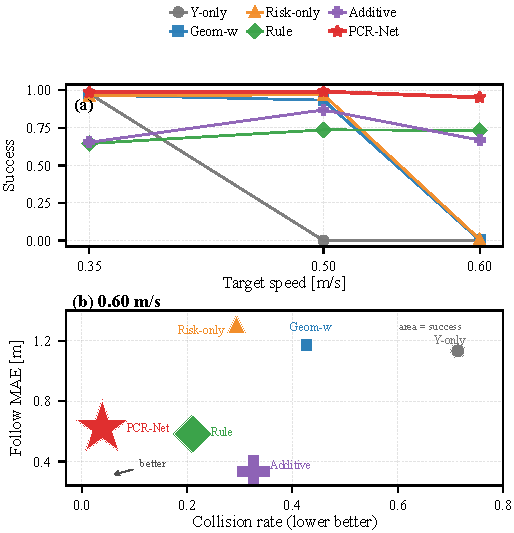
\includegraphics[width=\columnwidth]{figs/fig2_main_singlecol_compact.pdf}
\caption{Main performance at the fixed hardest stage. (a) Task success
vs.\ target speed. (b) Collision rate vs.\ follow MAE at $0.60\msec$ (point
area encodes task success; lower-left is better).}
\label{fig:main}
\end{figure}

\begin{figure*}[t]
\centering
\begin{minipage}[c]{0.35\textwidth}
\centering
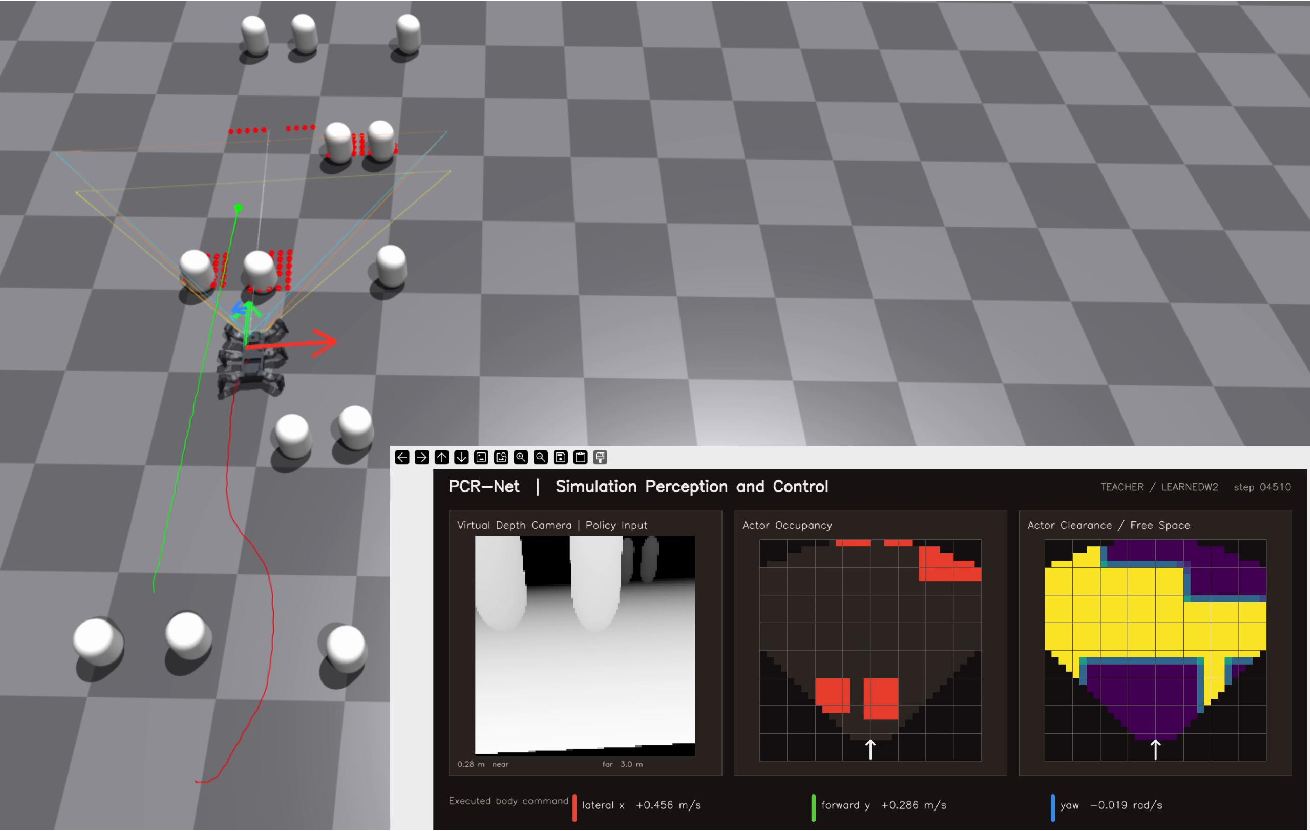
\includegraphics[width=\linewidth]{figs/fig5_sim_overview_crop.pdf}\\[-0.8mm]
{\scriptsize (a) Simulation scene and perception inputs.}
\end{minipage}\hfill
\begin{minipage}[c]{0.62\textwidth}
\centering
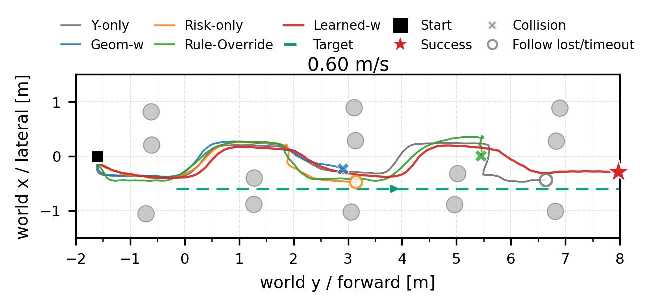
\includegraphics[width=\linewidth]{figs/fig6_traj.pdf}\\[-0.8mm]
{\scriptsize (b) Representative trajectories at $0.60\msec$.}
\end{minipage}
\caption{Simulation evidence at the hardest stage ($0.60\msec$).
(a) The obstacle-row scene and simulated perception inputs, including
occupancy and clearance maps. (b) Geom-w collides at the third row,
Risk-only loses the target near the third row, Rule-Override collides at
the fourth row, and Y-only reaches the final row but loses the target;
Learned-w alone clears all five rows and succeeds.}
\label{fig:simtraj}
\end{figure*}

\textbf{B. Inference ablation.}
Table~\ref{tab:mech} tests the learned correction by reusing the same
Learned-w checkpoint but forcing $\Delta y_w$ to zero only at inference,
leaving all else unchanged. Within the training range ($0.35$ and
$0.50\msec$), removing $\Delta y_w$ retains high task success; the collapse
appears only at the above-training speed
$0.60\msec$. At this speed, removing $\Delta y_w$ reduces row progress from
$0.985$ to $0.739$ and raises follow MAE from $0.623$ to
$1.463\,\mathrm{m}$, while collision is $0.133$. The ablated policy still
advances but cannot sustain the coordinated progress needed to maintain
follow distance through the final row; its dominant failure is therefore
loss of follow-distance regulation rather than collision. This
checkpoint-controlled ablation measures the trained composite policy's
dependence on $\Delta y_w$ and indicates that the learned correction supplies
the high-conflict margin needed for sustained following at the above-training
boundary.

\begin{table}[t]
\centering
\caption{Inference ablation of the learned correction: the same
Learned-w checkpoint is reused with $\Delta y_w$ forced to zero at
inference. $\Delta y_w$ is reported as predicted/used averages.}
\label{tab:mech}
\setlength{\tabcolsep}{2.5pt}
\scriptsize
\begin{tabular}{lccccc}
\toprule
Spd & Success $\uparrow$ & Row-prog. $\uparrow$ & Coll. $\downarrow$ & MAE [m] $\downarrow$ &
$\Delta y_w$ (pred./used) \\
\midrule
$0.35$ & $0.974$ & $0.993$ & $0.023$ & $0.176$ & $0.066/0$ \\
$0.50$ & $0.982$ & $0.992$ & $0.016$ & $0.438$ & $0.067/0$ \\
$0.60$ & $0.000$ & $0.739$ & $0.133$ & $1.463$ & $0.066/0$ \\
\bottomrule
\end{tabular}
\end{table}

\textbf{C. Structural alternative: Additive-Fusion.}
Does the orthogonal decomposition alone, without a learned gate, already
resolve the conflict? Additive-Fusion ($u=\uF+\uA$) preserves tracking well
(lowest follow MAE at $0.35$/$0.50\msec$) but collides far more ($0.344$,
$0.125$, $0.326$) and is unstable at high speed ($0.669$ success at
$0.60\msec$): preserving following is easy, but staying safe needs
context-dependent arbitration of how much avoidance to inject, which direct
addition lacks.
Fig.~\ref{fig:simtraj}(b) shows representative high-conflict trajectories.

\textbf{D. External alternatives.}
\label{sec:external}
We include two external alternatives with matched base observations, command
space, velocity limits, command post-processing, and fixed low-level policy.
Published leader-following and agile-navigation stacks often couple different
sensors, planners, and low-level controllers. We therefore use
interface-matched alternatives to isolate the arbitration design. Monolithic PPO also
matches PCR-Net in network capacity and training budget; the DWA-style search
uses validation-only tuned costs. They test whether a single learned policy or
hand-designed local search can replace learned command-space arbitration in
this benchmark.

\emph{Monolithic PPO.} As a structural alternative, we train a monolithic
PPO policy with the same base observations, matched backbone capacity,
and the same training budget as PCR-Net, but without the Follow/Avoid
decomposition, the directional risk query, or the gate; it predicts the
high-level command directly (Table~\ref{tab:mono}, evaluated at $0.35\msec$
over increasing row difficulty). It records only $0.093$/$0.064$ success at
Stages 2/3 and falls to $0.000$ at Stage 4, where collision reaches $1.000$;
the high Stage-4 FOV-in/L2 reflect short pre-collision episodes
(time-to-contact $1.51\,\mathrm{s}$), so the failure is early collision
rather than target loss. Under matched capacity and budget, the unstructured policy fails to form a
viable safety--progress baseline as row difficulty increases.

\begin{table}[t]
\centering
\caption{Monolithic PPO at fixed target speed $0.35\msec$ over increasing
obstacle-row difficulty.}
\label{tab:mono}
\setlength{\tabcolsep}{4pt}
\footnotesize
\begin{tabular}{lcccccc}
\toprule
Stage & Success $\uparrow$ & Row-prog. $\uparrow$ & Coll. $\downarrow$ &
FOV-in & L2 & TTC [s] \\
\midrule
2 & $0.093$ & $0.424$ & $0.445$ & $0.244$ & $0.180$ & $6.49$ \\
3 & $0.064$ & $0.322$ & $0.688$ & $0.313$ & $0.375$ & $4.21$ \\
4 & $0.000$ & $0.016$ & $1.000$ & $0.922$ & $0.898$ & $1.51$ \\
\bottomrule
\end{tabular}
\end{table}

\emph{DWA-style velocity search.} For the planner-style external baseline,
we implement a target-aware DWA-style velocity-space search under the same
local-map observation, relative-target state, high-level command space, and
shared post-processor as PCR-Net. It samples commands
$u=[u_x,u_y,u_\omega]$, applies a dynamic-window filter from the previous
command using acceleration limits, rolls out each reachable candidate on the
local map, rejects candidates whose footprint intersects occupied cells or
whose clearance falls below a margin, and scores the rest by risk, target
distance, bearing, progress, and command smoothness,
\begin{equation}
\begin{aligned}
J={}&\alpha_r J_{\mathrm{risk}}+\alpha_d J_{\mathrm{dist}}
+\alpha_b J_{\mathrm{bearing}}-\alpha_p J_{\mathrm{prog}}\\
&-\alpha_f J_{\mathrm{fwd}}+\alpha_s J_{\Delta u}+\alpha_l J_{\mathrm{lat}}.
\end{aligned}
\label{eq:dwa_cost}
\end{equation}
After validation-only tuning, all tests use a $7{\times}5{\times}5$ base
grid augmented with fixed near-zero velocity samples before dynamic-window
filtering; rollouts use a
$1.2\,\mathrm{s}$ horizon at $0.15\,\mathrm{s}$,
$0.32\,\mathrm{m}$ footprint, $0.08\,\mathrm{m}$ clearance margin, and
acceleration limits $(3.0,2.0,4.0)$ for forward, lateral, and yaw commands.
A finer $21{\times}11{\times}11$ resolution check gives the same qualitative
safety--progress trend at $4\times$ mean planning latency; we report the base
grid to satisfy the shared $10\,\mathrm{Hz}$ high-level control budget.
Unlike PCR-Net, this fixed-cost short-horizon search has neither learned
context-dependent arbitration nor distance-decayed risk memory;
Table~\ref{tab:dwa} tests its sufficiency in this matched benchmark, not
the broader DWA family.
The resulting comparison is reported in Table~\ref{tab:dwa}. In this
moving-target row-conflict setting, no fixed-cost setting yields a
stable safety--progress balance: success is at most $0.082$ at $0.35\msec$
and zero at $0.60\msec$, with collision $0.612$--$0.969$. The footprint
check is applied to nominal rollouts on the local grid, while contact is
measured after execution by the shared legged stack; short-horizon feasible
commands can therefore still lead to contact after replanning and tracking
dynamics. Safety bias suppresses progress yet remains collision-prone;
tracking-oriented costs increase progress without resolving collision.

\begin{table}[t]
\centering
\caption{DWA-style velocity-search alternative.}
\label{tab:dwa}
\setlength{\tabcolsep}{3pt}
\footnotesize
\begin{tabular}{llcccc}
\toprule
Search bias & Spd & Success $\uparrow$ & Coll. $\downarrow$ &
Row-prog. $\uparrow$ & MAE [m] $\downarrow$ \\
\midrule
\multirow{2}{*}{Safety-biased}
 & $0.35$ & $0.053$ & $0.612$ & $0.138$ & $0.678$ \\
 & $0.60$ & $0.000$ & $0.838$ & $0.000$ & $1.028$ \\
\multirow{2}{*}{Balanced}
 & $0.35$ & $0.026$ & $0.938$ & $0.188$ & $0.375$ \\
 & $0.60$ & $0.000$ & $0.969$ & $0.375$ & $0.592$ \\
\multirow{2}{*}{Tracking-biased}
 & $0.35$ & $0.082$ & $0.744$ & $0.344$ & $0.528$ \\
 & $0.60$ & $0.000$ & $0.881$ & $0.500$ & $0.690$ \\
\bottomrule
\end{tabular}
\end{table}

\textbf{E. Real-robot deployment.}
We deploy the policy on a hexapod in a cluttered corridor: a narrow indoor
corridor with two staggered obstacle rows whose passable space alternates
left and right, so the robot must sidestep into the open gap of each row
while keeping the walking person in view. Hardware rows replace the regular
simulated primitives with boxes and cones, providing direct evidence of
transfer beyond the simulated obstacle representation. The robot closes the loop with
onboard perception: YOLOv8 target detection~\cite{ref:yolo} provides the
relative goal; target-associated depth points are masked out before the
remaining stereo depth is rasterized into the two-channel
occupancy--free-space map.
Under the same staggered-row protocol, PCR-Net succeeds in $19/20$ trials
versus $12/20$ for Rule-Override, whose eight failures comprise six
collisions and two target-loss events (Table~\ref{tab:real}).
On these matched trials, PCR-Net reduces mean follow-distance MAE from $1.21$
to $0.52\,\mathrm{m}$ and raises mean executed forward speed from $0.32$ to
$0.51\msec$, indicating tighter tracking with more sustained progress.
The hardware deployment uses stereo-depth maps rather than the
actor-rasterized maps used in simulation, and the $60$-trial hardware evaluation
tests this deployed perception path directly; to reduce transient
perception loss the deployment adds a short obstacle-map memory to the
scalar risk memory of Sec.~IV-C.

Fig.~\ref{fig:real_arbitration} shows a representative logged real-robot
segment. Stereo-derived Follow-risk peaks lower the risk-only Follow weight,
and the learned correction partially restores $\yeff$ while keeping it below
the raw gate, so the net command remains avoidance-biased without fully
suppressing Follow. During these conflict intervals, the lateral command
rises while forward motion stays nonzero. The hardware trace complements the
high-conflict simulation in Fig.~\ref{fig:simtraj}(b): risk-conditioned
arbitration keeps forward motion active during lateral avoidance rather than
collapsing into a pure avoidance override.
Fig.~\ref{fig:real_views} shows the deployed robot sequence and the
corresponding onboard perception/local-map sequence.

\begin{figure}[t]
\centering
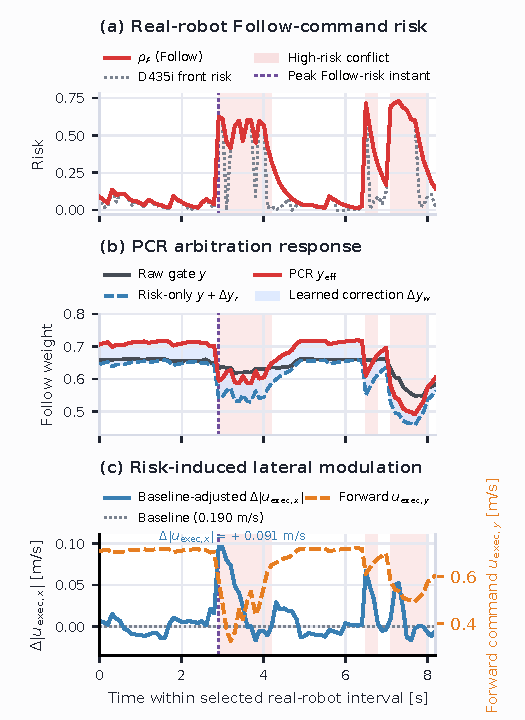
\includegraphics[width=\columnwidth]{figs/fig7_arbitration.pdf}
\caption{Representative real-robot arbitration trace. (a) Stereo-derived
risk peaks mark conflict intervals. (b) PCR lowers the risk-only Follow
response and the learned term partially restores $\yeff$. (c) The executed
command increases lateral motion while keeping forward motion nonzero.}
\label{fig:real_arbitration}
\end{figure}

\begin{figure*}[!t]
\centering
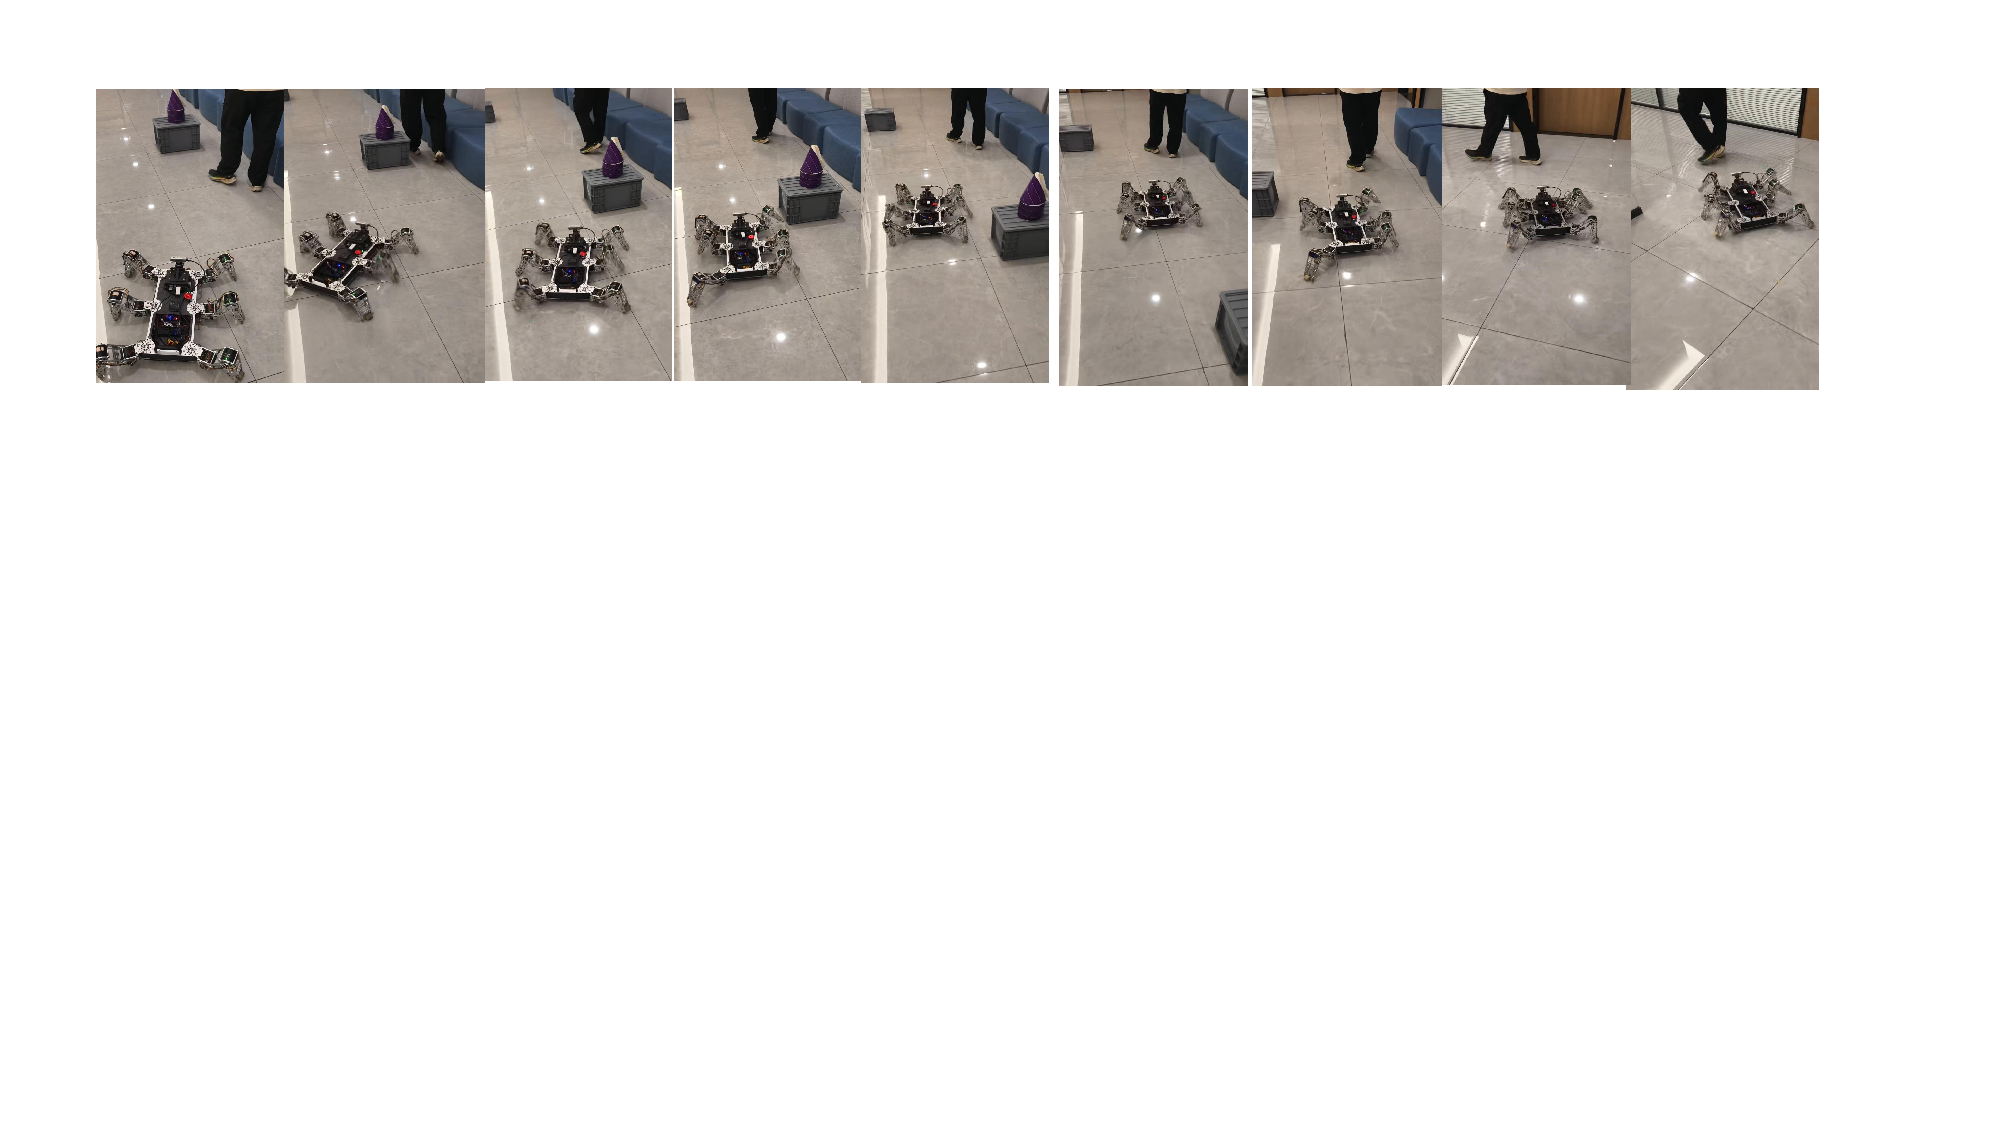
\includegraphics[width=\textwidth]{figs/fig4a_real_follow.pdf}\\[-1.8mm]
{\scriptsize (a) Third-person real-robot following sequence.}\\[-0.2mm]
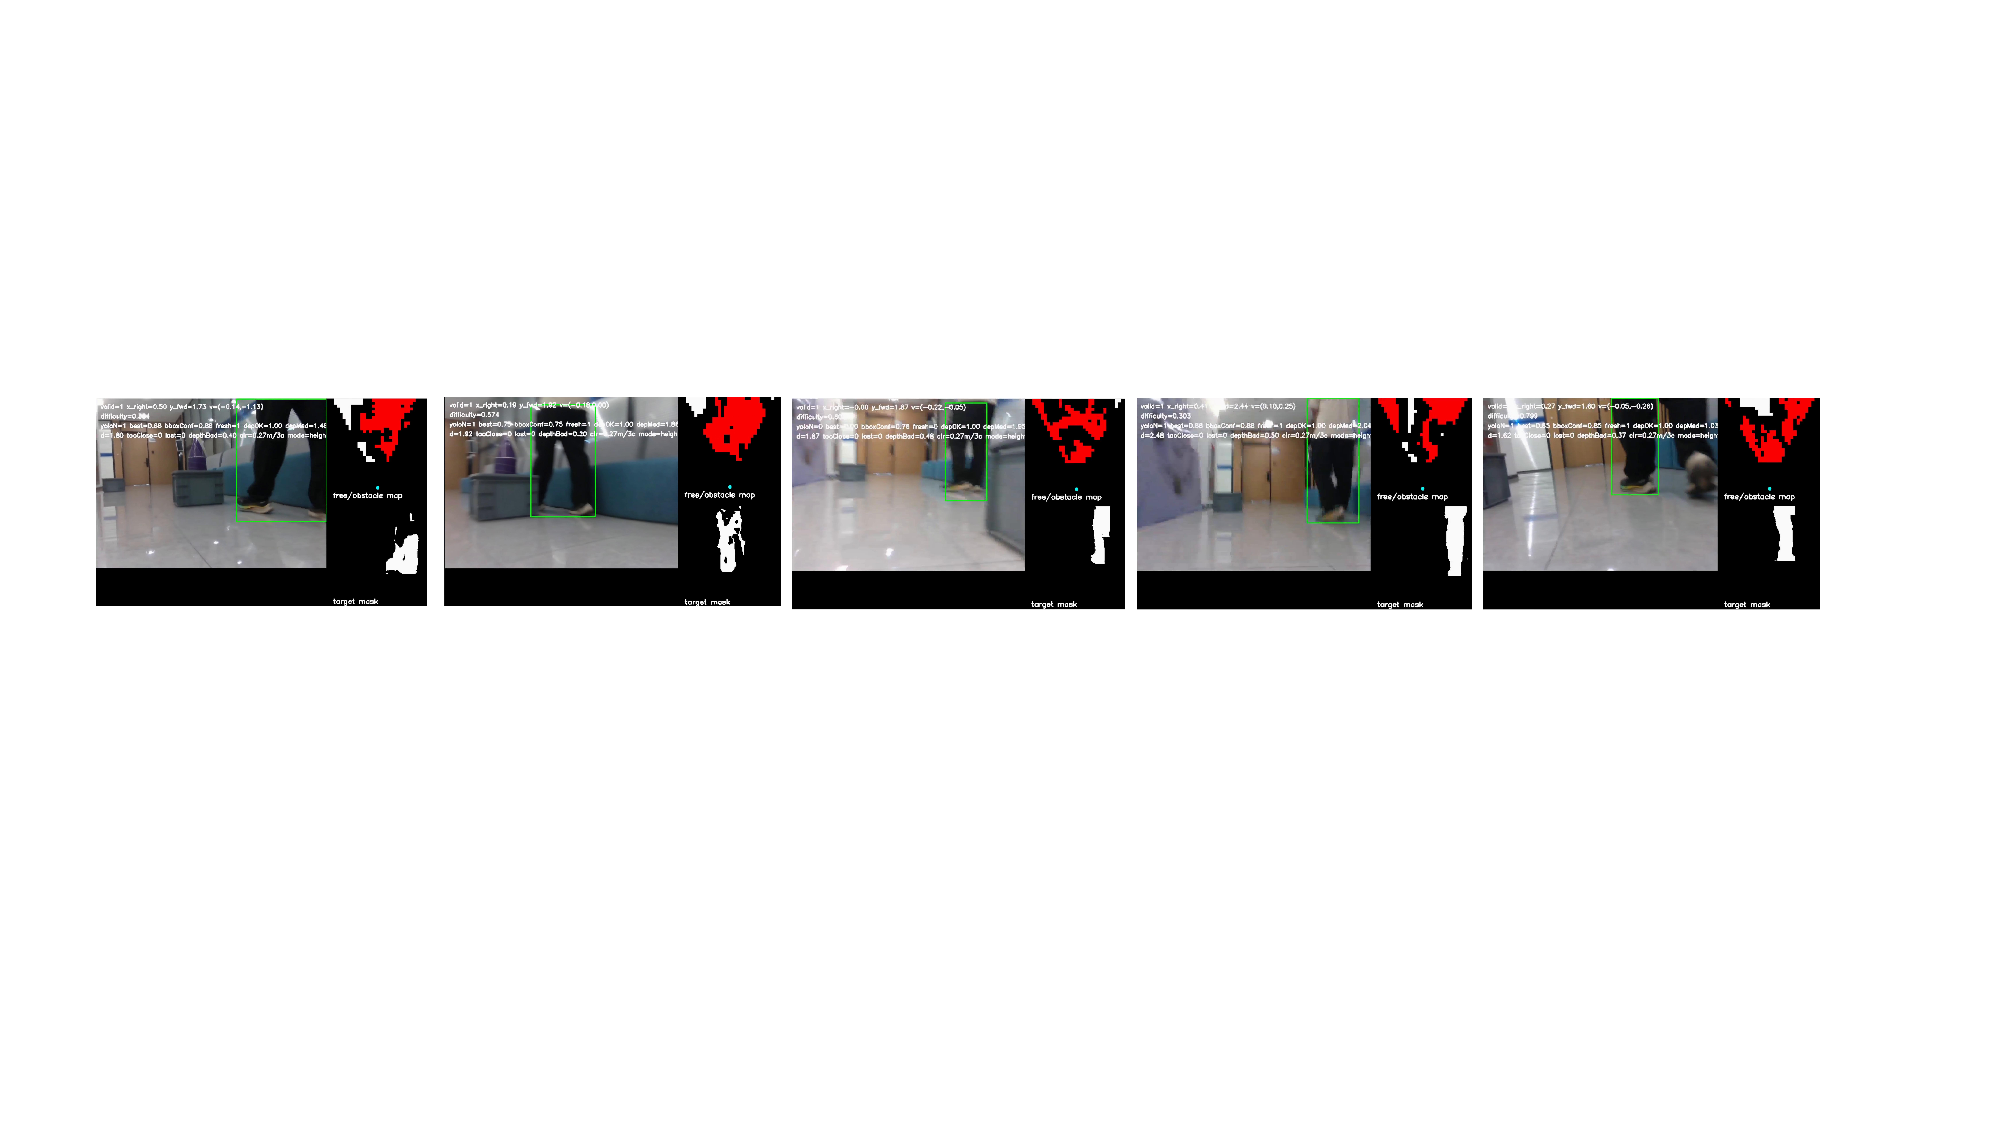
\includegraphics[width=\textwidth]{figs/fig4b_real_onboard.pdf}\\[-1.8mm]
{\scriptsize (b) Onboard target detection, stereo-depth view, and local-map sequence.}
\caption{Real-robot deployment views. (a) The hexapod follows the walking
target while sidestepping around staggered corridor obstacles. (b) The
onboard perception stream provides the target state and stereo-depth local
affordance map used by PCR-Net.}
\label{fig:real_views}
\end{figure*}

We additionally evaluate a more demanding corridor scene that requires a
sharp target turn between obstacle rows: the target exits the first row,
turns $90^\circ$, and enters a second row with a different traversal
direction. The same deployed policy succeeds in $18/20$ trials without
scene-specific switching, with failures from one glancing obstacle contact
and one target-loss event during the turn. The complete sharp-turn sequence
is included in the supplementary video. Across both scenes PCR-Net succeeds in $37/40$
trials, providing quantitative hardware evidence that the deployed
perception--arbitration--locomotion chain can operate on the real hexapod
under corridor clutter. Each hardware trial is scored at the episode
level: success requires completing the corridor segment without obstacle
contact or target loss.

\begin{table}[t]
\centering
\caption{Real-robot results over $60$ trials. Rule-Override uses staggered
rows; the sharp-turn scene joins two row segments at $90^\circ$.}
\label{tab:real}
\scriptsize
\begin{tabular*}{\columnwidth}{@{\extracolsep{\fill}}llccccc@{}}
\toprule
Method & Scene & Trials & Success & Coll. & Lost & Rate \\
\midrule
PCR-Net & Staggered rows & $20$ & $19$ & $1$ & $0$ & $95\%$ \\
Rule-Ov. & Staggered rows & $20$ & $12$ & $6$ & $2$ & $60\%$ \\
PCR-Net & Sharp target turn & $20$ & $18$ & $1$ & $1$ & $90\%$ \\
PCR-Net & Overall & $40$ & $37$ & $2$ & $1$ & $92.5\%$ \\
\bottomrule
\end{tabular*}
\end{table}

\section{Discussion and Limitations}
\textbf{Why it works.} PCR-Net retains following authority during lateral
avoidance. Removing $\Delta y_w$ reduces row progress and breaks
follow-distance regulation rather than primarily causing collision. The
alternatives expose complementary failures: additive fusion cannot regulate
avoidance authority, while fixed-cost velocity search finds no stable
safety--progress balance in this benchmark.

\textbf{Limitations and future work.}
Controlled simulation ablations use straight staggered rows, while the
sharp-turn hardware scene evaluates two row segments joined by a $90^\circ$
change in traversal direction, using the same deployed local-map policy
without scene-specific switching. The speed-scaled risk check supports the
simpler directional prior over the tested low-speed regime; braking-distance-
or trajectory-aware risk remains a natural extension for faster motion.

\section{Conclusion}
We formulated hexapod target following in clutter as command-space conflict
arbitration and proposed PCR-Net, a risk-conditioned gate that softly fuses
Follow/Avoid proposals over a fixed locomotion policy. Learned arbitration
gives the best tested safety--following balance, with inference ablation
identifying the high-conflict role of $\Delta y_w$. A $60$-trial hardware
evaluation ($40$ PCR-Net, $20$ Rule-Override) across straight and $90^\circ$
connected-row layouts supports the deployed perception--arbitration--locomotion
chain.

\begin{thebibliography}{99}
\setlength{\itemsep}{-1.2pt}
\bibitem{ref:personfollowing} M.~J. Islam, J.~Hong, and J.~Sattar,
``Person-following by autonomous robots: A categorical overview,'' \emph{The
International Journal of Robotics Research}, vol.~38, no.~14, pp.~1581--1618,
2019.
\bibitem{ref:leaderfollow} C.~Scheidemann \emph{et al.},
``Obstacle-avoidant leader following with a quadruped robot,'' in
\emph{2025 IEEE International Conference on Robotics and Automation (ICRA)},
2025, pp.~1407--1413.
\bibitem{ref:abs} T.~He, C.~Zhang, W.~Xiao, G.~He, C.~Liu, and G.~Shi,
``Agile but safe: Learning collision-free high-speed legged locomotion,'' in
\emph{Robotics: Science and Systems (RSS)}, 2024.
\bibitem{ref:miki} T.~Miki, J.~Lee, J.~Hwangbo, L.~Wellhausen, V.~Koltun,
and M.~Hutter, ``Learning robust perceptive locomotion for quadrupedal
robots in the wild,'' \emph{Science Robotics}, vol.~7, no.~62, p.~eabk2822,
2022.
\bibitem{ref:dwa} D.~Fox, W.~Burgard, and S.~Thrun, ``The dynamic window
approach to collision avoidance,'' \emph{IEEE Robotics \& Automation
Magazine}, vol.~4, no.~1, pp.~23--33, 1997.
\bibitem{ref:taskpriority} Y.~Nakamura, H.~Hanafusa, and T.~Yoshikawa,
``Task-priority based redundancy control of robot manipulators,'' \emph{The
International Journal of Robotics Research}, vol.~6, no.~2, pp.~3--15, 1987.
\bibitem{ref:cbf} A.~D. Ames, X.~Xu, J.~W. Grizzle, and P.~Tabuada,
``Control barrier function based quadratic programs for safety critical
systems,'' \emph{IEEE Transactions on Automatic Control}, vol.~62, no.~8,
pp.~3861--3876, 2017.
\bibitem{ref:reachavoid} K.-C. Hsu, V.~Rubies-Royo, C.~J. Tomlin, and
J.~F. Fisac, ``Safety and liveness guarantees through reach-avoid
reinforcement learning,'' in \emph{Robotics: Science and Systems (RSS)},
2021.
\bibitem{ref:moe} R.~A. Jacobs, M.~I. Jordan, S.~J. Nowlan, and
G.~E. Hinton, ``Adaptive mixtures of local experts,'' \emph{Neural
Computation}, vol.~3, no.~1, pp.~79--87, 1991.
\bibitem{ref:policyblend} A.~D. Dragan and S.~S. Srinivasa, ``A
policy-blending formalism for shared control,'' \emph{The International
Journal of Robotics Research}, vol.~32, no.~7, pp.~790--805, 2013.
\bibitem{ref:residualrl} T.~Johannink \emph{et al.}, ``Residual reinforcement
learning for robot control,'' in \emph{2019 IEEE International Conference on
Robotics and Automation (ICRA)}, 2019, pp.~6023--6029.
\bibitem{ref:yolo} G.~Jocher, A.~Chaurasia, and J.~Qiu, ``Ultralytics
YOLOv8,'' Ultralytics, 2023. [Online]. Available:
\url{https://github.com/ultralytics/ultralytics}
\bibitem{ref:rudin} N.~Rudin, D.~Hoeller, P.~Reist, and M.~Hutter,
``Learning to walk in minutes using massively parallel deep reinforcement
learning,'' in \emph{Proceedings of the 5th Conference on Robot Learning
(CoRL)}, 2022, pp.~91--100.
\bibitem{ref:ppo} J.~Schulman, F.~Wolski, P.~Dhariwal, A.~Radford, and
O.~Klimov, ``Proximal policy optimization algorithms,'' \emph{arXiv
preprint arXiv:1707.06347}, 2017.
\bibitem{ref:isaac} V.~Makoviychuk \emph{et al.}, ``Isaac Gym:
High-performance GPU-based physics simulation for robot learning,'' in
\emph{NeurIPS Datasets and Benchmarks Track}, 2021.
\end{thebibliography}

\end{document}
